\documentclass[11pt,letterpaper]{article}
\usepackage[T1]{fontenc}
\usepackage[utf8]{inputenc}
\usepackage{lmodern}
\usepackage[margin=1in,headheight=15pt]{geometry}
\usepackage{amsmath,amssymb,amsthm,mathtools}
\usepackage{graphicx,booktabs,array,longtable}
\usepackage{microtype,setspace,fancyhdr,titlesec,caption,xurl}
\usepackage[hidelinks,unicode]{hyperref}
\usepackage[section]{placeins}
\setstretch{1.04}
\setlength{\parindent}{0pt}
\setlength{\parskip}{5pt}
\setlength{\emergencystretch}{2em}
\titleformat{\section}{\large\bfseries}{\thesection.}{.5em}{}
\titleformat{\subsection}{\normalsize\bfseries}{\thesubsection.}{.5em}{}
\titlespacing*{\section}{0pt}{2.1ex plus 1ex minus .2ex}{.9ex}
\titlespacing*{\subsection}{0pt}{1.7ex plus .7ex minus .2ex}{.6ex}
\captionsetup{font=small,labelfont=bf,skip=7pt}
\pagestyle{fancy}\fancyhf{}
\fancyhead[L]{\small\itshape Binary graph embeddings and SI metric reconstruction}
\fancyhead[R]{\small P. Leblond}
\fancyfoot[C]{\thepage}
\renewcommand{\headrulewidth}{.3pt}
\newtheorem{theorem}{Theorem}[section]
\newtheorem{proposition}[theorem]{Proposition}
\newtheorem{corollary}[theorem]{Corollary}
\theoremstyle{definition}
\newtheorem{definition}[theorem]{Definition}
\newtheorem{example}[theorem]{Example}
\theoremstyle{remark}
\newtheorem{remark}[theorem]{Remark}
\newcommand{\E}{\mathbb E}
\newcommand{\Prob}{\mathbb P}
\newcommand{\R}{\mathbb R}
\newcommand{\one}{\mathbf 1}
\newcommand{\dSI}{d_{\mathrm{SI}}}
\newcommand{\dhat}{\widehat d_K}
\newcommand{\diag}{\operatorname{diag}}
\newcommand{\Geom}{\operatorname{Geom}}
\newcommand{\Exp}{\operatorname{Exp}}
\newcommand{\rank}{\operatorname{rank}}
\newcommand{\tr}{\operatorname{tr}}
\newcommand{\corr}{\operatorname{corr}}
\newcommand{\specnorm}[1]{\left\lVert #1\right\rVert_{\mathrm{op}}}
\newcommand{\norm}[1]{\left\lVert #1\right\rVert}
\newcommand{\SImeanGof}{0.9151}
\newcommand{\SIsdGof}{0.0005}
\newcommand{\SImeanGap}{18.53}
\newcommand{\SImeanNeg}{0.0346}
\newcommand{\SImeanCoord}{0.0354}

\hypersetup{pdftitle={Collapse of Binary Graph Embeddings and Metric Reconstruction via SI First-Passage Dynamics},pdfauthor={Philippe Leblond},pdfsubject={Weighted graph metrics, first-passage percolation, multidimensional scaling}}
\title{\LARGE\bfseries Collapse of Binary Graph Embeddings\\and Metric Reconstruction via\\SI First-Passage Dynamics\\[.6em]\large\mdseries Weighted audits, conditional recovery, and reproducible MDS calibration}
\author{Philippe Leblond\\\small\texttt{leblond.philippe@gmail.com}}
\date{September 30, 2026\\\small Research draft}
\begin{document}
\maketitle
\begin{abstract}
Binary shortcut metrics can obscure an underlying spatial geometry, but their failure is not a universal collapse to rank two. We separate distance contraction, shell counting, loss of low-dimensional spectral concentration, and finite-sample reconstruction error. Exact counterexamples show that complete-graph hop metrics have rank $N-1$, while rescaled binary paths converge to a continuous interval. The useful necessity statement is therefore conditional: continuously adjustable coupling on a fixed graph requires state beyond binary adjacency, not a rejection of every unweighted continuum limit.

We formulate a reference-based weighted audit and construct an SI first-passage estimator by averaging shortest-path metrics over shared random edge fields. Every finite-sample estimate is a metric; independently sampled source rows, even after symmetrization, need not be. We prove recovery of the intact-backbone mean metric when a finite set of added shortcut probabilities tends to zero, and give an explicit perturbation bound connecting metric recovery to classical multidimensional scaling (MDS).

New computations improve the two-dimensional positive-spectral-mass score of a $10\times10$ grid from $0.7749$ to $0.9151$, with sample standard deviation $0.0005$ across five Monte Carlo replications. A three-dimensional control also improves. However, uniform SI does not remove the radial mode of finite-box Delaunay graphs. A coordinate-length oracle sharply reduces that distortion but is not an intrinsic reconstruction rule. Weighted coarsening, D11 tail diagnostics, and disk-interface curvature are consequently assigned their precise, distinct evidential roles rather than treated as a completed proof of universal manifold reconstruction.
\end{abstract}
\noindent\textbf{Keywords:} weighted graph metrics; susceptible--infectious dynamics; first-passage percolation; multidimensional scaling; metric audits; geometric reconstruction.

\section{Introduction}
A graph does not determine a unique operational notion of distance. Hop count treats all present edges as equally traversable; a weighted shortest-path metric assigns heterogeneous traversal costs; an infection process measures arrival times generated by repeated interactions. These constructions may produce different volume profiles and different MDS spectra on the same adjacency structure. A reconstruction claim must therefore identify the metric being reconstructed, the variables carrying its information, and the reference against which its error is assessed.

The preceding paper, \emph{Distance, Volume, and Apparent Dimension in Weighted Graphs}, separated pointwise metric contraction, ball-volume inflation, and changes in fitted growth slopes \cite{leblond2026a}. This companion study adds a spectral reconstruction layer and a stochastic operational metric. Its starting point is the research program recorded in the \texttt{cursor/d1-dynamics-u-2031} branch of \texttt{alltoall-black-holes} \cite{leblondBranch}. The branch's labels D10, D10b, D11, and Tier-1 are retained to make the correspondence explicit; they are project identifiers, not mathematical dimensions or theorem numbers.

Three distinctions control the argument. First, a failure to recover a two-dimensional reference is not evidence that a graph has collapsed \emph{into} a two-dimensional state. In the grid controls, two dominant MDS modes are a desired null signature. Second, a continuous metric can arise as a rescaled limit of binary graphs. The motivation for weighted microscopic state is the ability to express heterogeneous or continuously tunable interactions on a fixed topology, not an impossibility theorem for all binary constructions. Third, SI first passage belongs to established stochastic growth and first-passage percolation, rather than constituting a new general propagation mechanism \cite{richardson1973,vandenberg1993}. The contribution here is its integration with metric-preserving estimation, explicit recovery conditions, and an audit that detects misleading geometric conclusions.

Classical scaling reconstructs a Euclidean configuration from squared distances when its centered Gram matrix is positive semidefinite \cite{schoenberg1935}. Graph-based manifold learning likewise requires assumptions connecting graph distances to a relevant continuum metric; the graph-to-geodesic step is not justified by the final embedding alone \cite{tenenbaum2000}. Perturbation theory makes this separation quantitative: a good embedding follows from controlled distance errors and suitable spectral conditioning, not merely from choosing an output dimension \cite{arias2020}.

The paper has three parts. Part I supplies exact diagnostics and counterexamples for binary metrics. Part II states the weighted audit, its prospective registration requirements, and what a finite coarsening pilot actually demonstrates. Part III gives the SI construction and recovery theorem, followed by finite-dimensional calibration and deliberately retained negative controls. All newly tabulated simulations were executed with the accompanying independent implementation. Historical D11 observations are clearly marked as source-reported rather than newly reproduced.

\section{Metrics, spectra, and evidential conventions}\label{sec:notation}
Let $V$ be a finite labeled set, $N=|V|\geq2$, and let $d_0$ be a reference metric. A connected, undirected graph $G=(V,E)$ with strictly positive edge costs $\ell_e$ induces
\begin{equation}
 d_\ell(x,y)=\min_{P:x\leadsto y}\sum_{e\in P}\ell_e.
 \label{eq:shortest}
\end{equation}
We distinguish a coupling strength $g_e$, a deterministic traversal cost $\ell_e$, a discrete transmission probability $p_e$, and a continuous-time transmission rate $\beta_e$. None of these quantities is identified with another without specifying a conversion rule and its units. The notation $L_0$ refers to the microscopic graph-description level of the research program, not the $\ell_0$ sparsity functional.

For any symmetric dissimilarity matrix $D$ with zero diagonal, classical MDS forms
\begin{equation}
 J=I-\frac1N\one\one^{\mathsf T},\qquad
 B(D)=-\frac12 JD^{\circ2}J,
 \label{eq:gram}
\end{equation}
where $D^{\circ2}$ denotes entrywise squaring. Let $\lambda_1\geq\cdots\geq\lambda_N$ be the eigenvalues of $B$. When at least $d$ eigenvalues are positive, the $d$-coordinate output is $Y_d=U_d\diag(\sqrt{\lambda_1},\ldots,\sqrt{\lambda_d})$. This construction optimizes a Gram-matrix approximation criterion; it does not automatically minimize distance stress.

We report complementary diagnostics:
\begin{align}
 G_d&=\frac{\sum_{i=1}^d\max(\lambda_i,0)}{\sum_{i=1}^N\max(\lambda_i,0)}, &
 g_{d,d+1}&=\frac{\lambda_d}{\lambda_{d+1}},\label{eq:diagnostics1}\\
 \eta_-&=\frac{\sum_{\lambda_i<0}|\lambda_i|}{\sum_{\lambda_i>0}\lambda_i}, &
 r_+&=\frac{(\sum_{\lambda_i>0}\lambda_i)^2}{\sum_{\lambda_i>0}\lambda_i^2}.
 \label{eq:diagnostics2}
\end{align}
The eigengap ratio is reported only when the denominator is positive; an exact absence of further positive modes is denoted by $\infty$. The participation ratio $r_+$ is an effective count of positive modes, not algebraic rank. The separate positive rank is $n_+=\#\{i:\lambda_i>0\}$. Numerical zero conventions are given in Appendix~\ref{app:repro}.

For a known calibration configuration $X$, centered at its centroid, we also use
\begin{equation}
 E_X^{(d)}=\min_{a\geq0,\,Q^{\mathsf T}Q=I}
 \frac{\norm{aY_dQ-X}_F}{\norm{X}_F},\qquad
 S_d=\frac{\norm{\Delta(Y_d)-D}_F}{\norm{D}_F},
 \label{eq:errors}
\end{equation}
where $\Delta(Y_d)$ is its Euclidean distance matrix. Translation is removed by centering, and the coordinate comparison permits one global scale and an orthogonal transformation, including reflection. Coordinates are used only for evaluation or for explicitly labeled oracle controls. A metric-only spectral score is not substituted for coordinate error.

\part*{Part I. Diagnostic: what binary metrics do and do not imply}

\section{The shell-counting dilemma is a bookkeeping problem}\label{sec:shell}
Consider the nearest-neighbor square lattice with its unit hop metric and an interior source. Before a finite boundary is reached, its shell and ball are
\begin{equation}
 S_r=\{(i,j):|i|+|j|=r\},\qquad B_r=\bigcup_{s=0}^r S_s.
\end{equation}

\begin{proposition}[Shell, volume, and cut counts]\label{prop:shell}
For an integer $r\geq1$,
\begin{equation}
 |S_r|=4r,\qquad |B_r|=1+2r(r+1),\qquad
 |\partial_E B_r|=8r+4.
 \label{eq:shell}
\end{equation}
Moreover,
\begin{equation}
 \sum_{r=0}^{R}|B_r|=(R+1)+\frac23R(R+1)(R+2).
 \label{eq:doublecount}
\end{equation}
The cubic growth in \eqref{eq:doublecount} counts repeated memberships, not new vertices.
\end{proposition}
\begin{proof}
There are four axial shell vertices and $4(r-1)$ nonaxial vertices. Summing the shell counts gives the ball volume. Each nonaxial boundary vertex has two outward edges and each axial boundary vertex has three, giving $2(4r-4)+12=8r+4$. Summing the resulting quadratic ball formula proves \eqref{eq:doublecount}. A vertex at distance $s\leq R$ occurs in the balls $B_s,\ldots,B_R$, exactly $R-s+1$ times. Thus the sum of cumulative volumes cannot be interpreted as a count of independent newly accessible vertices.
\end{proof}

Adding a shortcut can change which vertices belong to a shell, as well as its size. It does not make shortest-path computation incorrect: the hop algorithm still computes the metric defined by the modified adjacency. The error arises when that metric is interpreted as preserving an earlier spatial geometry without testing the interpretation. Similarly, counting all pairs in a shell does not by itself establish that every pair represents an independent microscopic degree of freedom. Such a conclusion needs an operational state space and its constraints.

Table~\ref{tab:shells} illustrates another distinction. The shell-restricted Manhattan distance matrices retain approximately constant leading two-mode mass while their positive algebraic rank grows. Stable spectral concentration is therefore not a proof of constant rank, and a growing number of shell vertices is not a proof of an additional spatial dimension.
\begin{table}[htbp]
\centering
\begin{tabular}{rrrrrr}
\toprule
$r$ & $|S_r|$ & $|B_r|$ & $G_2$ & $n_+$ & $r_+$ \\
\midrule
5 & 20 & 61 & 0.772 & 11 & 3.112 \\
8 & 32 & 145 & 0.772 & 16 & 3.121 \\
11 & 44 & 265 & 0.772 & 23 & 3.125 \\
14 & 56 & 421 & 0.772 & 28 & 3.127 \\
\bottomrule
\end{tabular}

\caption{New exact-distance shell calculations. Distances are measured through the ambient square lattice, not along the shell perimeter. $n_+$ grows while $G_2$ and $r_+$ remain approximately stable.}
\label{tab:shells}
\end{table}

\section{Binary shortcuts and the loss of geometric information}\label{sec:binary}
\subsection{A complete graph rules out a universal rank-two collapse}
The maximally shortcut-rich binary graph provides an exact diagnostic.
\begin{theorem}[Equidistance gives high rank]\label{thm:complete}
Let every off-diagonal distance on $N$ vertices equal $c>0$. Then
\begin{equation}
 B=\frac{c^2}{2}J.
\end{equation}
There are $N-1$ positive eigenvalues, all equal to $c^2/2$, and one zero eigenvalue. Consequently, for $1\leq d\leq N-1$,
\begin{equation}
 G_d=\frac{d}{N-1},\qquad r_+=N-1.
 \label{eq:complete}
\end{equation}
In particular, the hop metric of $K_N$ has no distinguished two-dimensional eigenspace.
\end{theorem}
\begin{proof}
The squared-distance matrix is $c^2(\one\one^{\mathsf T}-I)$. Since $J\one=0$ and $J^2=J$, equation~\eqref{eq:gram} yields the stated result. The action of $J$ is the identity on $\one^\perp$ and zero on the constant vector.
\end{proof}

This is a collapse of spatial contrast, not a collapse of algebraic rank. For large $N$, a fixed-dimensional projection retains a vanishing fraction of the positive spectral mass. Its selected coordinates depend on arbitrary choices within a highly degenerate eigenspace. The full metric instead realizes an $(N-1)$-dimensional equilateral simplex.

\begin{proposition}[A quantitative near-equidistance regime]\label{prop:flat}
Suppose $B\one=0$ and
\begin{equation}
 \specnorm{B-\tfrac{c^2}{2}J}\leq\varepsilon<c^2/2.
\end{equation}
Then all $N-1$ eigenvalues on $\one^\perp$ are positive and belong to $[c^2/2-\varepsilon,c^2/2+\varepsilon]$. In particular,
\begin{equation}
 G_d\leq
 \frac{d(c^2/2+\varepsilon)}{(N-1)(c^2/2-\varepsilon)}.
 \label{eq:flatbound}
\end{equation}
\end{proposition}
\begin{proof}
For any unit $v\perp\one$, the Rayleigh quotient $v^{\mathsf T}Bv$ differs from $c^2/2$ by at most $\varepsilon$. The extremal eigenvalue characterization bounds every centered eigenvalue. Bounding the numerator above and the positive spectral sum below gives \eqref{eq:flatbound}.
\end{proof}

The hypothesis is explicit: the proposition is not a theorem that every shortcut perturbation must approach equidistance. One nearby shortcut can be benign, while a sufficiently disruptive collection can erase useful separation between modes. The effect depends on endpoint placement, reference geometry, and metric costs.

There is also an identifiability obstruction. If a reconstruction rule uses only adjacency and is equivariant under relabeling, its output dissimilarity on $K_N$ must be invariant under every permutation. Hence all off-diagonal output distances agree. It cannot recover a particular non-equilateral arrangement whose labels and spatial distinctions have already been erased. A successful recovery then requires additional state, measurements, or assumptions.

\subsection{A new degree-preserving damage benchmark}
We independently construct a $20\times20$ grid and attempt one or ten degree-preserving edge swaps with seed zero. At each attempt, two edges with four distinct endpoints are replaced by crossed edges when no duplicate would result. Node ordering, edge ordering, and the realized graph are recorded in the supplement. An edge is classified as a topological ``long'' when, after deleting that edge, its endpoints cannot be reconnected in at most three hops. This definition is graph-internal and differs from counting only the newly inserted edges.

All fabric-class edges retain cost one. Long-class edges receive a common cost $\ell_{\rm long}\in\{1,2,5,20\}$. The unchanged grid hop metric is the reference. Table~\ref{tab:static} includes an exhaustive all-center arrival-event volume audit, not just a central-source curve.
\begin{table}[htbp]
\centering\small
\begin{tabular}{rrrrrrrr}
\toprule
Swaps & $\ell_{\rm long}$ & Longs & $G_2$ & $g_{23}$ & $r_+$ & $\max R$ & Bad edges \\
\midrule
0 & 1 & 0 & 0.769 & 6.82 & 3.32 & 1.00 & 0 \\
1 & 1 & 3 & 0.768 & 6.79 & 3.32 & 1.25 & 2 \\
10 & 1 & 27 & 0.357 & 1.32 & 10.39 & 3.96 & 20 \\
10 & 2 & 27 & 0.380 & 1.40 & 9.59 & 3.05 & 19 \\
10 & 5 & 27 & 0.471 & 1.82 & 7.22 & 1.77 & 18 \\
10 & 20 & 27 & 0.759 & 6.32 & 3.39 & 1.10 & 1 \\
\bottomrule
\end{tabular}

\caption{New static-distance benchmark. ``Bad edges'' satisfy $\ell_{uv}<d_0(u,v)$. The maximum volume ratio is taken over all 400 centers and every event radius. The ten-swap graph contains 27 detour-classified longs. These are newly generated results, not a transcription of the branch's historical 30-long fixture.}
\label{tab:static}
\end{table}

The one-swap example barely changes $G_2$, despite producing endpoint contractions. Ten swaps reduce $G_2$ from $0.769$ to $0.357$ and raise $r_+$ from $3.32$ to $10.39$. That is a loss of two-dimensional dominance, not its creation. Increasing the long cost to 20 restores much of the spectral concentration, but one underpriced edge and 3,332 contracted unordered pairs remain. A favorable MDS picture therefore does not certify pointwise metric recovery.

\begin{figure}[htbp]
\centering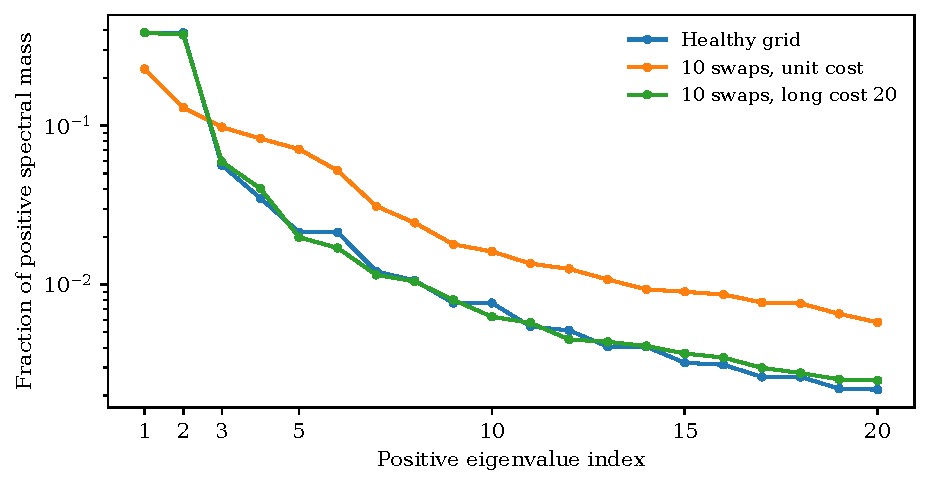
\includegraphics[width=.89\linewidth]{figures/damage_spectrum.pdf}
\caption{Positive MDS spectra in the new damage benchmark. Unit-cost shortcuts spread mass across many modes. High long-edge costs restore a strong leading pair without making every reference-distance comparison correct.}
\label{fig:damage}
\end{figure}

\section{What the weighted \texorpdfstring{$L_0$}{L0} claim can legitimately establish}\label{sec:continuum}
\begin{proposition}[An unweighted continuum counterexample]\label{prop:path}
Let $P_n$ be the binary path on vertices $0,\ldots,n$ and equip it with the rescaled hop metric $d_n(i,j)=|i-j|/n$. The map $i\mapsto i/n$ is an isometry into $[0,1]$. Its image has Hausdorff distance at most $1/(2n)$ from the interval. Thus binary paths, after a common change of units, approximate a continuous spatial metric arbitrarily well.
\end{proposition}
\begin{proof}
The unique path from $i$ to $j$ has $|i-j|$ edges. Every point of the interval is within $1/(2n)$ of a grid vertex, including the endpoints. Both conclusions follow directly.
\end{proof}

Likewise, a uniformly rescaled nearest-neighbor lattice approximates the continuous $\ell_1$ metric on a box of any fixed dimension. This metric is not Euclidean, but it is continuous and its underlying topology is the usual box topology. Therefore the universal statement that unweighted or combinatorial models cannot support continuous spatial metrics is false. Even the binary-path example already defeats it.

A narrower statement is useful. For fixed finite $V$, there are only finitely many simple binary adjacency matrices. A deterministic adjacency-only rule consequently has only finitely many outputs. It cannot encode a nonconstant continuously varying family of coupling states while the topology remains fixed. A weighted state $G=(V,E,g)$ supplies such a parameter space, but it is not the only logically possible extension: interaction-time distributions, additional vertex variables, or distributions over graphs also carry nonbinary information.

The operational advantage of weighted $L_0$ state is therefore flexibility and testability. A present edge can become weak without being deleted, and its effect can be audited as its microscopic interaction parameter changes. What remains to be derived in a physical application is why a particular local state determines a particular cost or propagation law. That derivation cannot be replaced by selecting weights that yield a preferred MDS dimension.

\part*{Part II. Weighted audits, registration, and coarse-graining}

\section{The D10 weighted-audit protocol}\label{sec:audit}
Fix a strictly positive vertex measure $\mu$ common to the candidate and reference. Define closed-ball volumes
\begin{equation}
 V_d(x,r)=\sum_{v\in V}\mu(v)\one\{d(x,v)\leq r\},\qquad
 R_x(r)=\frac{V_d(x,r)}{V_{d_0}(x,r)}.
 \label{eq:volume}
\end{equation}
The center is included, so the denominator is positive for $r\geq0$. The audit proceeds from the metric definition to edge comparisons, complete arrival profiles, and only then slope or embedding summaries. This extends the workflow of the first paper and its implementation in the research branch \cite{leblond2026a,leblondWeighted}.

\begin{proposition}[Deterministic edge-cost certificate]\label{prop:domination}
For the metric \eqref{eq:shortest},
\begin{equation}
 d_\ell(x,y)\geq d_0(x,y)\ \text{for every }x,y
 \quad\Longleftrightarrow\quad
 \ell_{uv}\geq d_0(u,v)\ \text{for every }uv\in E.
 \label{eq:certificate}
\end{equation}
An underpriced edge is an endpoint witness to contraction. If, in addition, every edge and cost of a reference realization $G_0$ is retained, then \eqref{eq:certificate} implies $d_\ell=d_0$.
\end{proposition}
\begin{proof}
If all edge inequalities hold, the reference triangle inequality bounds every candidate path cost below by $d_0(x,y)$. Conversely, $d_\ell(u,v)\leq\ell_{uv}$, so an underpriced edge violates domination at its endpoints. With an intact reference realization, its original shortest paths also give $d_\ell\leq d_0$, proving equality.
\end{proof}

The last hypothesis matters: making the added edges expensive cannot reconstruct edges that a degree-preserving swap removed. It also matters that the certificate concerns deterministic costs. Section~\ref{sec:meantrap} shows why applying it to mean random edge times does not certify the mean SI metric.

For a finite source profile, $V_d$ and $V_{d_0}$ are step functions. Comparing them at the union of their arrival radii certifies their ordering on every interval between successive events. An integer-radius grid may miss fractional-radius excesses. A single-source audit certifies only that source; it cannot be silently promoted to a graph-wide statement. In the new static benchmark, all 400 sources are audited.

The three primary outputs remain distinct: endpoint contraction witnesses, maximal ball-volume ratios with their source/radius witnesses, and MDS reconstruction diagnostics. Common counting measure is used in the supplied experiments. Coarse-grained applications must instead state whether block mass equals one or the sum of constituent masses; those conventions produce different volume observables.

\section{Weight selection and prospective pre-registration}\label{sec:prereg}
A reconstruction audit cannot establish that a weight law was selected independently of the desired reconstruction. That independence is a design requirement. Before a confirmatory run, a registration should fix the allowed microscopic variables, the cost/probability map, all tunable parameters, graph generators, random seeds or seed policy, reference metrics, calibration windows, boundary treatment, and failure criteria.

A general local candidate might have the form
\begin{equation}
 p_{uv}=\min\{1,p_\star f_\theta(\chi_u,\chi_v,\mathcal N_{uv})\},
 \qquad f_\theta>0,
 \label{eq:genericrule}
\end{equation}
where $\mathcal N_{uv}$ is a specified local graph neighborhood and $\chi$ is an independently defined microscopic variable. Equation~\eqref{eq:genericrule} is a protocol template, not a derived law or a rule validated here. Its parameters cannot be retuned on the evaluation graphs to maximize $G_2$, remove a third mode, or match target coordinates. Any conservation law $Q$, update operator $U$, and map from state to interaction probability must be stated separately; conservation of a sum of numerical edge weights is not assumed merely because the weights exist.

The primary computations in this draft use a frozen execution configuration, \texttt{code/design.json}, written before their execution. The probability $p=1/2$ is transferred without optimization. A secondary configuration, \texttt{extension\_design.json}, was specified after the initial batch and before the dimension-control and Delaunay-SI transfer runs. Those secondary results are diagnostic, not a previously registered confirmatory test. Neither file was deposited in an external, time-stamped registration service. A hash fixes file contents; it does not prove an earlier public commitment.

Two forms of privileged information are explicitly retained as controls. The weak-shortcut experiment knows which edges were added by its generator, and the Euclidean-length oracle knows the evaluation coordinates. These controls test mathematical mechanisms and attainable reconstruction quality. Neither is offered as a method for discovering unknown physical edge weights from adjacency alone.

\section{What the weighted-RG pilot establishes}\label{sec:rg}
We examine the branch-inspired static coarsening rule separately from SI dynamics. A $40\times40$ grid undergoes 20 connected degree-preserving swaps. Vertices are grouped into coordinate-labeled $2\times2$ blocks; internal edges are discarded, and parallel interblock edges are merged using either their minimum or their mean cost. Nodes are retained even if no crossing edge remains. Coordinates here define the blocking apparatus; this is not an intrinsic graph-only blocking construction.

At each level, the coarsened pristine grid supplies a unit-hop reference. A coarse edge has span $s_e=d_0(u,v)$ and is called long when $s_e>1$. We report
\begin{equation}
 \lambda_{\rm long}=\frac{\#\{e:s_e>1\}}{|E|},\qquad
 \Phi=\frac{\#\{e:s_e>1,\ \ell_e<s_e\}}{\#\{e:s_e>1\}}.
 \label{eq:rgobs}
\end{equation}
Initial long costs are 1, 3, or 10; other edges have unit cost. Figure~\ref{fig:rg} and Table~\ref{tab:rg} report new realizations rather than asserting exact agreement with earlier version-dependent swap outputs.

\begin{table}[htbp]
\centering
\begin{tabular}{rrrrrr}
\toprule
Level & $N$ & $|E|$ & $\lambda_{\rm long}$ & $\Phi$ & $\langle\ell/s\rangle_{\rm long}$ \\
\midrule
0 & 1600 & 3120 & 0.013 & 0.900 & 0.500 \\
1 & 400 & 793 & 0.042 & 0.636 & 1.096 \\
2 & 100 & 210 & 0.143 & 0.133 & 1.902 \\
3 & 25 & 56 & 0.286 & 0.000 & 2.938 \\
\bottomrule
\end{tabular}

\caption{New minimum-cost coarsening pilot with initial long cost 10. The reference span is measured in the unit grid at each level, without rescaling inherited costs. Topological long-edge prevalence grows while underpricing eventually vanishes.}
\label{tab:rg}
\end{table}

\begin{figure}[htbp]
\centering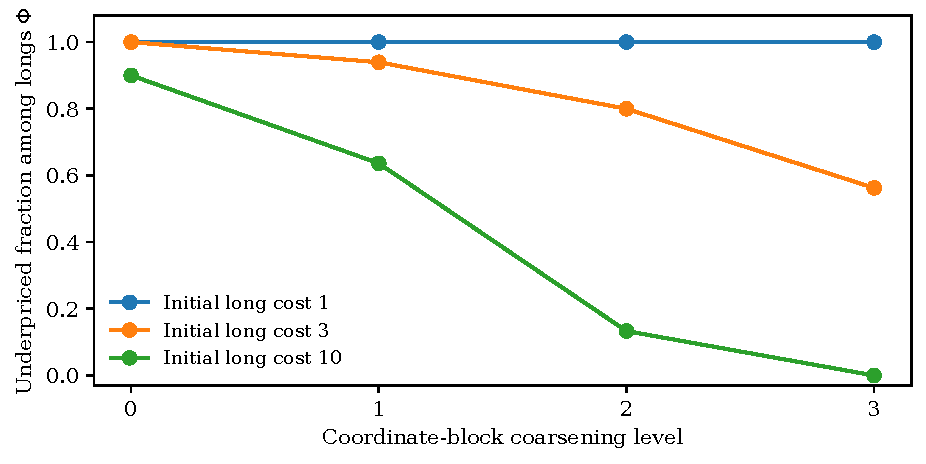
\includegraphics[width=.86\linewidth]{figures/rg_pricing.pdf}
\caption{Static pricing flow under the same coordinate-block minimum rule. Unit-cost longs remain underpriced. Long cost 10 becomes noncontracting relative to the coarse reference by level three. This is not a measurement of an RG eigenvalue.}
\label{fig:rg}
\end{figure}

The minimum rule keeps all span-one fabric edges at unit cost in this realization. The flow of $\Phi$ nevertheless depends strongly on the initial prices. Its disappearance at the final $5\times5$ grid for long cost 10 has an elementary explanation: the largest reference Manhattan span is only eight. Inherited long costs have not been rescaled with that shrinking span. The observation demonstrates conditional price washout under a specified convention, not scale invariance of the full metric or a universal fixed point.

A genuine RG claim would additionally specify the length and time rescalings, vertex-mass transformation, treatment of internal block traversal, retained effective interactions, and a convergent family of coarse observables. None follows from freezing a favorable merger rule. In particular, a static minimum-cost merger is not automatically the coarse operator for stochastic SI.

\begin{proposition}[Parallel SI channels do not merge by mean-cost minimization]\label{prop:parallel}
If parallel channels connect the same already active source to the same susceptible target, with independent exponential transmission times of rates $\beta_1,\ldots,\beta_m$, their earliest arrival has rate $\sum_i\beta_i$. For synchronous independent Bernoulli attempts, the one-step effective success probability is $1-\prod_i(1-p_i)$.
\end{proposition}
\begin{proof}
The probability that no exponential clock rings by time $t$ is $\prod_i e^{-\beta_i t}=e^{-t\sum_i\beta_i}$. In discrete time, a step fails precisely when every independent attempt fails.
\end{proof}

Thus the exponential mean passage time is $1/\sum_i\beta_i$, not $\min_i(1/\beta_i)$. General block aggregation also includes internal arrival delays and correlations. Unless an appropriate closure or time-scale separation is established, the effective coarse dynamics need not remain in the same independent-edge SI family.

\part*{Part III. SI first passage and conditional metric reconstruction}

\section{A dynamical metric with a metric-preserving estimator}\label{sec:si}
\subsection{Persistent SI and random edge passage times}
In the discrete SI process, one source is infected at time zero. During each subsequent step, every infected vertex attempts to infect each susceptible neighbor independently with probability $p_e\in(0,1]$. Infected vertices remain infectious, and newly infected vertices become active on the next step. This is a persistent epidemic front, not a single random walker and not an algorithm that discards a transmitter after a failed attempt. The source branch implements this repeated-attempt convention \cite{leblondSI}.

For each undirected edge, draw an independent passage time
\begin{equation}
 \tau_e\sim\Geom(p_e),\qquad
 \Prob(\tau_e=k)=(1-p_e)^{k-1}p_e,\quad k=1,2,\ldots.
 \label{eq:geom}
\end{equation}
Define the realized first-passage distance
\begin{equation}
 T_\tau(x,y)=\min_{P:x\leadsto y}\sum_{e\in P}\tau_e,
 \qquad \dSI(x,y)=\E[T_\tau(x,y)].
 \label{eq:fpp}
\end{equation}
For a fixed source, this random shortest-path construction has the same infection-time law as persistent SI with symmetric edge probabilities. One may defer sampling an edge's waiting time until its first endpoint becomes infected; the edge then waits for its first successful independent Bernoulli attempt. Independence of unexposed edge variables and the minimum-arrival recursion produce \eqref{eq:fpp}. This equivalence does not assert that separately simulated sources must share the same physical epidemic realization.

The continuous-time analogue uses $\tau_e\sim\Exp(\beta_e)$. The discrete construction has the pathwise lower bound $T_\tau\geq d_{\rm hop}$. Exponential waiting times have no strictly positive deterministic lower bound per edge, so a finite-speed causal cone cannot be inferred from them without additional assumptions. In neither formulation does an operational arrival metric by itself establish a relativistic causal geometry.

\subsection{The common-field estimator}
\begin{theorem}[Metric preservation at every sample size]\label{thm:metric}
Let $G$ be finite, connected, and undirected. Suppose each edge time is strictly positive almost surely and has finite expectation. Then $T_\tau$ and $\dSI$ are metrics. For independent, identically distributed field samples $\tau^{(1)},\ldots,\tau^{(K)}$, the estimator
\begin{equation}
 \dhat(x,y)=\frac1K\sum_{k=1}^K T_{\tau^{(k)}}(x,y)
 \label{eq:estimate}
\end{equation}
is a metric for every $K\geq1$, and converges almost surely to $\dSI$ simultaneously for every vertex pair as $K\to\infty$.
\end{theorem}
\begin{proof}
Each realization is a positive shortest-path metric: paths can be reversed, distinct vertices require positive total length, and concatenating paths proves the triangle inequality. The graph has finitely many simple paths, so the minimum is strictly positive for distinct endpoints. A fixed connecting path bounds $T_\tau$ above by a finite sum of integrable edge times. Hence the expectation exists and is finite. Taking expectations preserves symmetry and triangle inequalities; a strictly positive integrable random variable has positive expectation. A finite convex average has the same properties. The strong law applies to each pair, and the intersection of finitely many probability-one convergence events still has probability one.
\end{proof}

The implementation draws one undirected edge field per trial, computes its all-pairs shortest paths, and accumulates the resulting matrix. It uses no target coordinates, spectral projection, or triangle-repair operation. Shared fields introduce dependence \emph{between} pair estimates, while each pair still has the correct marginal mean. That dependence is intentional: it preserves the inequalities jointly.

\begin{example}[Symmetric independently sampled rows need not form a metric]\label{ex:rows}
On the path $a-b-c$, consider three independent one-trial source runs. From $a$, let the two successive edge waits be $(1,3)$; from $b$, let both waits be one; from $c$, let the successive waits be $(1,3)$. All events have positive probability under \eqref{eq:geom} when $0<p<1$. The assembled row matrix is
\begin{equation}
 M=\begin{pmatrix}0&1&4\\1&0&1\\4&1&0\end{pmatrix}.
\end{equation}
It is already symmetric, but $M_{ac}=4>M_{ab}+M_{bc}=2$. Symmetrization alone does not repair it.
\end{example}

The branch's original estimator averages independently simulated source rows and then symmetrizes \cite{leblondSI}. Its large-sample population target is the same under the homogeneous, symmetric assumptions above, but its finite-sample geometry and random-number coupling differ from \eqref{eq:estimate}. The new numerical scores below must therefore not be described as exact reruns of its historical $K=100$ regression.

The supplied sampler has no finite-time infection cap. On a connected graph with $p_e>0$, geometric edge times are finite almost surely and every sampled distance is finite. A simulator that stops at a cap must report censoring rather than silently treating an unreached vertex as having arrived at the cap. Disconnected graphs are rejected by the present all-pairs implementation.

\section{Mean edge costs do not certify the SI metric}\label{sec:meantrap}
The dynamic construction is not obtained by simply replacing each random edge time by its expectation. For any fixed path $P$,
\begin{equation}
 \E\min_Q\sum_{e\in Q}\tau_e
 \leq\E\sum_{e\in P}\tau_e.
\end{equation}
Minimizing the right-hand side gives
\begin{equation}
 d_{\rm hop}(x,y)\leq\dSI(x,y)\leq d_{\E\tau}(x,y)
 \quad\text{for geometric passage times}.
 \label{eq:jensen}
\end{equation}
The left inequality is particular to the support $\{1,2,\ldots\}$. The right inequality also holds for exponential or other integrable positive times. Alternative paths lower expected first arrival through random competition, even when every individual mean edge time is large.

\begin{example}[A triangle defeats a mean-cost domination argument]\label{ex:triangle}
Take a triangle with independent geometric edge times of parameter $p=1/2$. Let $X$ be the direct edge wait and $Y,Z$ the two waits along the alternative route. Then $\E X=\E Y=\E Z=2$, but
\begin{equation}
 \E\min(X,Y+Z)=\frac{16}{9}<2.
 \label{eq:triangle}
\end{equation}
Thus mean edge costs dominate the equilateral reference metric with off-diagonal distance two, while the mean SI metric does not.
\end{example}
\begin{proof}
Put $q=1-p$. For integer $t\geq0$,
\begin{equation}
 \Prob(X>t)=q^t,\qquad
 \Prob(Y+Z>t)=q^t+tpq^{t-1},
\end{equation}
with the second term zero at $t=0$. The latter event is that at most one success has occurred in $t$ Bernoulli trials. Independence and the integer tail-sum formula give
\begin{equation}
 \E\min(X,Y+Z)=\frac{1}{1-q^2}+
 \frac{pq}{(1-q^2)^2}.
\end{equation}
Substitution of $p=q=1/2$ yields $4/3+4/9=16/9$.
\end{proof}

For exponential mean-one waits, the analogous expectation is $3/4$: integrate $e^{-2t}(1+t)$ from zero to infinity. The issue is therefore not a peculiarity of discrete time. Proposition~\ref{prop:domination} can be applied realization by realization when $\tau_{uv}\geq d_0(u,v)$ almost surely. That stronger assumption gives $T_\tau\geq d_0$ pathwise and hence $\dSI\geq d_0$. A lower bound on $\E\tau_{uv}$ alone does not.

There is a second expectation-order distinction. The volume of a ball in the mean metric,
\begin{equation}
 \sum_v\mu(v)\one\{\E T_\tau(x,v)\leq t\},
\end{equation}
is generally different from the expected infected mass,
\begin{equation}
 \E\sum_v\mu(v)\one\{T_\tau(x,v)\leq t\}
 =\sum_v\mu(v)\Prob(T_\tau(x,v)\leq t).
 \label{eq:infectedmass}
\end{equation}
A D10 or D11 comparison must specify which object it uses. Averaging a distance matrix before constructing its balls and averaging infection-front volumes are distinct experiments.

\section{Conditional restoration by weakening shortcuts}\label{sec:recovery}
A useful recovery statement is possible without assuming a continuum limit or a preferred output dimension.
\begin{theorem}[Finite-graph weak-shortcut recovery]\label{thm:recovery}
Let $G_0=(V,E_0)$ be a finite connected graph whose edge probabilities $p_e^0\in(0,1]$ remain fixed. Add a finite edge set $E_+$ without deleting or altering reference edges. Suppose the added probabilities $p_e(\varepsilon)>0$ tend to zero as $\varepsilon\downarrow0$. Let $\dSI^\varepsilon$ and $\dSI^0$ be the respective mean geometric first-passage metrics. Then
\begin{equation}
 \max_{x,y\in V}\left|\dSI^\varepsilon(x,y)-\dSI^0(x,y)\right|\longrightarrow0.
 \label{eq:recovery}
\end{equation}
Under a common-field coupling, every realized distance converges to the intact-backbone distance. If the added probabilities decrease monotonically, these realized distances increase monotonically toward that limit.
\end{theorem}
\begin{proof}
Use the same reference edge times in both graphs. For every added edge choose an independent $U_e\in(0,1)$ and set
\begin{equation}
 \tau_e^\varepsilon=\left\lceil
 \frac{\log U_e}{\log(1-p_e(\varepsilon))}\right\rceil,
 \label{eq:coupling}
\end{equation}
with the usual deterministic value one when $p_e=1$. This gives the geometric law and $\tau_e^\varepsilon\to\infty$ almost surely. For any realization, the intact graph has finite random diameter $M_0=\max_{x,y}T_0(x,y)$. Because $E_+$ is finite, eventually every added edge costs more than $M_0$. No minimizing path can then use an added edge, since an intact path of cost at most $M_0$ is available for every pair. Thus $T_\varepsilon=T_0$ simultaneously for all pairs beyond a realization-dependent threshold.

For all $\varepsilon$, $0\leq T_\varepsilon(x,y)\leq T_0(x,y)$. The latter is integrable, so dominated convergence yields convergence of each mean distance. Finitely many pairs give \eqref{eq:recovery}. Monotone decrease of the probabilities makes every coupled added waiting time nondecreasing, and shortest-path distances inherit that monotonicity.
\end{proof}

The conclusion restores the \emph{reference SI metric}, not necessarily Euclidean distance. It also does not cover swap damage unless a connected reference realization remains intact. Finally, its quantifiers keep $N$ and $|E_+|$ fixed. With a growing number of weak channels, their collective effect can persist; an infinite-network or joint large-$N$ limit requires additional control. For example, the probability that any one of $m$ geometric shortcut waits is at most a fixed horizon $t$ is at most $t\sum_{e\in E_+}p_e$ by a union bound. This bound illustrates why per-edge weakness and aggregate weakness need not agree.

\subsection{A coupled numerical recovery experiment}
The experiment adds eight edges to a $10\times10$ grid, retaining all original edges. Their endpoint reference spans are at least eight hops, with generator seed 17. Reference edges use $p_0=1/2$, and added edges use $p_+=0.5/a$ for $a\in\{1,4,20,100\}$. The same 512 uniform edge fields are coupled across all values of $a$ and the intact control using \eqref{eq:coupling}. We measure
\begin{equation}
 E_D(a)=\frac{\norm{\widehat D(a)-\widehat D(\infty)}_F}{\norm{\widehat D(\infty)}_F}.
 \label{eq:relmetric}
\end{equation}
The reference in this expression is the coupled Monte Carlo intact metric, not the exact population mean. Its use removes irrelevant between-run noise when demonstrating the monotone mechanism.

\begin{table}[htbp]
\centering
\begin{tabular}{rrrrrr}
\toprule
$a$ & $p_{\rm long}$ & $E_D$ & $G_2$ & $g_{23}$ & $E_X$ \\
\midrule
1 & 0.500 & 0.3404 & 0.5641 & 1.73 & 0.6375 \\
4 & 0.125 & 0.2184 & 0.6348 & 1.96 & 0.3954 \\
20 & 0.025 & 0.0822 & 0.7926 & 4.78 & 0.1296 \\
100 & 0.005 & 0.0192 & 0.8912 & 13.69 & 0.0423 \\
$\infty$ & 0.000 & 0.0000 & 0.9158 & 18.15 & 0.0330 \\
\bottomrule
\end{tabular}

\caption{New shared-field weak-shortcut experiment. $a=\infty$ denotes the intact graph with no effective added transmission. All finite-$a$ matrices remain metrics. Residual geometric error is reported rather than rounded into a recovery claim.}
\label{tab:weak}
\end{table}

\begin{figure}[htbp]
\centering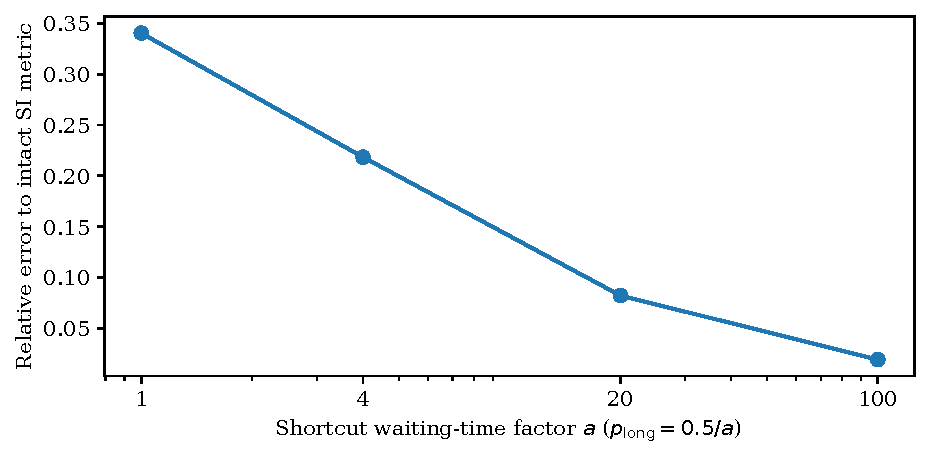
\includegraphics[width=.86\linewidth]{figures/weak_shortcut_recovery.pdf}
\caption{Relative metric error decreases as added interactions weaken. The finite-sample curve is an illustration of Theorem~\ref{thm:recovery}, not an estimate of a universal scaling exponent.}
\label{fig:weak}
\end{figure}

The observed error falls from $0.3404$ to $0.0192$. Meanwhile $G_2$ rises from $0.5641$ to $0.8912$, compared with $0.9158$ for the intact sampled metric. The strongest suppression therefore approaches, but does not equal, the reference. No assertion of exact finite-weight restoration is needed.

\section{From metric control to MDS control}\label{sec:perturbation}
\begin{theorem}[An explicit finite-$N$ Gram perturbation bound]\label{thm:perturbation}
Let $D_0,D$ be symmetric zero-diagonal nonnegative distance matrices with $\max_{ij}(D_0)_{ij}\leq M$ and $\max_{ij}|D_{ij}-(D_0)_{ij}|\leq\delta$. Then
\begin{equation}
 \specnorm{B(D)-B(D_0)}\leq
 \frac N2\delta(2M+\delta)=:\varepsilon_B.
 \label{eq:grambound}
\end{equation}
If $D_0$ is a Euclidean distance matrix with centered Gram rank $d$ and $\lambda_d(B(D_0))>2\varepsilon_B$, the leading $d$ eigenvalues of $B(D)$ exceed $\varepsilon_B$ and every remaining eigenvalue has absolute value at most $\varepsilon_B$.
\end{theorem}
\begin{proof}
Entrywise,
\begin{equation}
 |D_{ij}^2-(D_0)_{ij}^2|
 \leq\delta(2M+\delta).
\end{equation}
The operator norm of a matrix is at most its Frobenius norm, which here is at most $N\delta(2M+\delta)$. Multiplication by the orthogonal projector $J$ cannot increase the operator norm, proving \eqref{eq:grambound}. The extremal eigenvalue characterization bounds every eigenvalue perturbation by $\varepsilon_B$. The unperturbed leading $d$ eigenvalues are positive and all remaining ones are zero, which gives the stated separation.
\end{proof}

For fixed $N$, Theorems~\ref{thm:recovery} and \ref{thm:perturbation} imply convergence of SI Gram matrices and their spectra in the weak-shortcut limit. If the baseline has a separated positive $d$-dimensional eigenspace, its MDS configuration is recovered up to orthogonal ambiguity. Quantitative Procrustes results with sharper conditioning and norm dependence are available in the established perturbation literature \cite{arias2020}.

The bound is sufficient, not necessary, and its factor of $N$ can be loose. Most importantly, it does not prove its own premise that $D_0$ is close to a Euclidean metric. That geometric approximation requires a separate sampling, propagation, or homogenization argument. Positive passage times and metric axioms alone do not supply it: on a tree with uniform $p$, unique paths give $\dSI=d_{\rm hop}/p$. A branching tree therefore remains a tree metric, not a smooth Euclidean sheet, after SI averaging.

\section{Tier-1 MDS calibration on known-dimensional controls}\label{sec:tier1}
\subsection{The square-grid control}
For the $10\times10$ open grid, we use $p=1/2$, $K=256$ shared fields, and five independent generator seeds $0,\ldots,4$. Each trial produces an all-pairs metric; exhaustive triangle checks find no positive violation in the averaged matrices. Because geometric times are integers and $K$ is a power of two, these stored averages are exactly representable as binary fractions at the scales used.

\begin{table}[htbp]
\centering
\begin{tabular}{lrrrrr}
\toprule
Metric & $G_2$ & $g_{23}$ & $\eta_-$ & $S_2$ & $E_X$ \\
\midrule
Hop & 0.7749 & 6.75 & 0.2965 & 0.1275 & 0.1034 \\
SI mean & 0.9151 & 18.53 & 0.0346 & 0.0452 & 0.0354 \\
SI sample SD & 0.0005 & 0.47 & 0.0012 & 0.0006 & 0.0009 \\
\bottomrule
\end{tabular}

\caption{New square-grid calibration. The SI mean and sample standard deviation summarize five independent Monte Carlo estimators on the \emph{same graph}. They are not variability estimates over graph ensembles, and they are not confidence intervals for an asymptotic dimension.}
\label{tab:si}
\end{table}

The mean two-mode mass is $\SImeanGof$ with sample standard deviation $\SIsdGof$, the mean eigengap ratio is $\SImeanGap$, and the negative-to-positive spectral mass ratio is $\SImeanNeg$. The mean coordinate error falls to $\SImeanCoord$, from $0.1034$ for hop distance. Both the metric-only and coordinate-based diagnostics improve. Negative spectral mass remains nonzero, so the estimated mean distance matrices are not exactly two-dimensional Euclidean distance matrices.

\begin{figure}[htbp]
\centering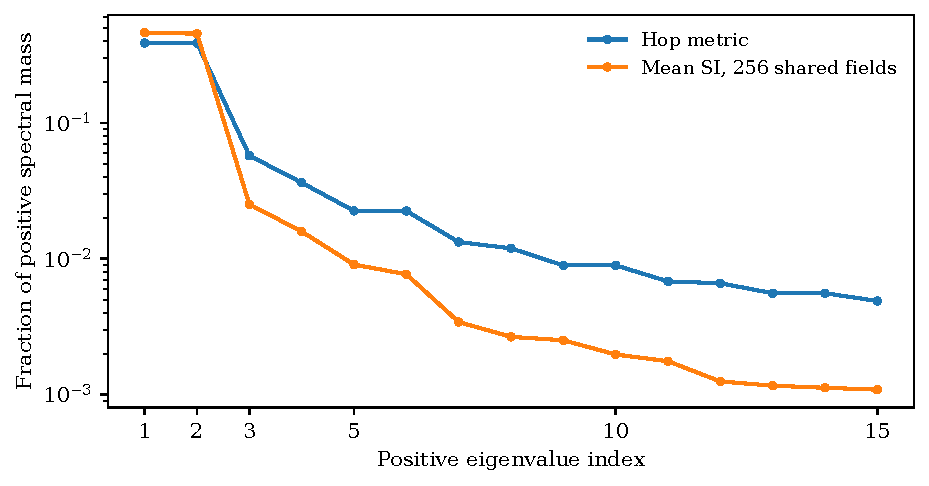
\includegraphics[width=.89\linewidth]{figures/si_spectrum.pdf}
\caption{Square-grid positive spectra for hop distance and one shared-field SI estimate. The improved separation is a finite calibration result. The retained small modes and negative eigenvalues rule out an exact rank-two claim.}
\label{fig:si}
\end{figure}

The historical branch also tests an SI grid improvement \cite{leblondMDS}. The present estimator changes both the sampling coupling and the trial count, so its better numerical score cannot be attributed to the coupling alone. Establishing a variance advantage would require a matched-budget comparison, which is not claimed here.

\subsection{One- and three-dimensional controls}
The secondary diagnostic batch transfers the same $p=1/2$ without tuning to a 100-vertex path and a $6^3$ cubic grid, with a $10\times10$ grid as the two-dimensional control. Every SI calculation uses 256 shared fields and seed 31415. The requested MDS dimension is the known dimension of the fixture, rather than a dimension inferred by selecting the best fit after observing its spectrum.
\begin{table}[htbp]
\centering
\begin{tabular}{rrlrrr}
\toprule
$d$ & $N$ & Metric & $G_d$ & $g_{d,d+1}$ & $E_X^{(d)}$ \\
\midrule
1 & 100 & hop & 1.0000 & $\infty$ & 0.0000 \\
1 & 100 & SI & 1.0000 & $\infty$ & 0.0040 \\
2 & 100 & hop & 0.7749 & 6.75 & 0.1034 \\
2 & 100 & SI & 0.9138 & 16.79 & 0.0363 \\
3 & 216 & hop & 0.7358 & 5.28 & 0.1065 \\
3 & 216 & SI & 0.8624 & 10.63 & 0.0532 \\
\bottomrule
\end{tabular}

\caption{New diagnostic controls in known dimensions. The path is exactly Euclidean for hop distance; a shared-field average remains a path metric and hence exactly one-dimensional, but its sampled edge means need not be perfectly uniform. The cubic grid improves under SI without becoming exactly rank three.}
\label{tab:dimensions}
\end{table}

For the cubic grid, $G_3$ increases from $0.7358$ to $0.8624$ and the three-coordinate error decreases from $0.1065$ to $0.0532$. Its three leading modes are approximately degenerate, so applying a universal two-mode criterion would incorrectly penalize a valid three-dimensional control. These results support finite-$d$ calibration on selected known geometries. They neither derive spatial dimension from an unspecified microscopic ensemble nor demonstrate a manifold limit as mesh size tends to zero.

A Tier-1 acceptance statement should identify the reference dimension, a metric approximation tolerance, coordinate or held-out distance error, spectral residuals, and boundary diagnostics. No single threshold for $G_2$ can replace that collection of tests across different dimensions and substrates.

\section{D11: tail identification is not a propagation-rate closure}\label{sec:d11}
The branch's D11 tests use deterministic weighted shortest paths and compare finite-window volume slopes around a modified central region \cite{leblondDimTests}. They do not implement a tension-dependent SI transmission exponent. Their source-reported diagnostics include an approximately constant $Er^2/100\in[0.633,0.642]$ for one weak-tension fixture and $Er\in[6.12,6.67]$ for another. A stronger fixture exhibits a drifting fitted exponent near $1.19$ versus $1.10$ in later windows. These values are \emph{archival source reports, not new runs in this supplement}; notably, the first normalization includes division by 100.

The appropriate mathematical object is the volume ratio from \eqref{eq:volume}. Let $p_d$ and $p_0$ be secant log-slopes on the same positive radii $r_1<r_2$. Then
\begin{equation}
 p_d-p_0=
 \frac{\log R_x(r_2)-\log R_x(r_1)}{\log(r_2/r_1)}.
 \label{eq:ratioidentity}
\end{equation}
The same subtraction identity holds for linear least-squares slopes on matched log-radius samples. Thus a positive slope excess can describe recovery of a volume deficit rather than inflation above the reference \cite{leblond2026a}.

For a differentiable interpolation with $R_x(r)=1-D_x(r)>0$,
\begin{equation}
 E(r)=\frac{d\log R_x}{d\log r}
 =-\frac{rD_x'(r)}{1-D_x(r)}.
 \label{eq:deficit}
\end{equation}
If one additionally assumes $D_x(r)=Ar^{-q}$ over a specified range, then
\begin{equation}
 E(r)=\frac{qAr^{-q}}{1-Ar^{-q}}.
 \label{eq:tailmodel}
\end{equation}
Equation~\eqref{eq:tailmodel} is conditional algebra, not a derivation of a universal exponent. Finite graph volumes are step functions; differentiability and any asymptotic power law require an explicitly stated approximation or limit.

A fitted response exponent $q$ is not the same object as a rate-law parameter $\alpha$ in, for example, $p_e=p_0(1+\chi_e)^{-\alpha}$. No equality between them follows from \eqref{eq:tailmodel}. Choosing $\alpha$ until an observed tail disappears would be calibration to the answer, not an independently predicted closure.

A defensible D11 closure would first fix the propagation law, then measure complete arrival-event volume ratios and matched slopes, distinguish balls of a mean metric from mean infected mass, and test the proposed tail on larger domains with boundary clearance. The project ledger explicitly calls for a ratio-based reanalysis \cite{leblondLedger}. The current evidence supports finite-window tail diagnostics; it does not establish elimination of long-range SI distortion.

\section{D10b: what the disk curvature confirmation measures}\label{sec:disk}
The D10b disk fixture is a dense inclusion inside a square-grid fabric, not an isolated flat disk reconstructed from SI times. We independently form the 29 grid vertices satisfying $(x-10)^2+(y-10)^2\leq9$ in a $20\times20$ grid. One fixture makes these vertices a clique. A milder fixture adds only king-move diagonals within the same disk.

For an edge $uv$, let $m_u$ and $m_v$ be the uniform measures on the neighbors of $u$ and $v$, with zero idleness. Using hop distance as the transport ground metric, compute Ollivier curvature \cite{ollivier2009}:
\begin{equation}
 \kappa(u,v)=1-\frac{W_1(m_u,m_v)}{d_{\rm hop}(u,v)}.
 \label{eq:curvature}
\end{equation}
Here $W_1$ is obtained by an exact finite transport linear program, solved numerically to solver tolerance. Internal edges have both endpoints in the inclusion; boundary edges have exactly one; all remaining edges are classified as fabric.

\begin{table}[htbp]
\centering\small
\begin{tabular}{llrrrr}
\toprule
Plug & Edge class & $n$ & Mean $\kappa$ & Minimum & Maximum \\
\midrule
Clique & internal & 15 & 0.898 & 0.742 & 0.964 \\
Clique & boundary & 15 & -0.791 & -1.242 & -0.556 \\
Clique & fabric & 15 & 0.000 & 0.000 & 0.000 \\
King & internal & 15 & -0.008 & -0.300 & 0.333 \\
King & boundary & 15 & -0.203 & -0.333 & -0.167 \\
King & fabric & 15 & 0.000 & 0.000 & 0.000 \\
\bottomrule
\end{tabular}

\caption{New disk-interface curvature measurements. Fifteen edges per class are sampled with Python's seed-zero generator; the exact sampled edges and individual curvatures are saved. This sampling differs from the historical NumPy-seeded fixture. Zero fabric means concern the sampled edges, not every outer-boundary edge of the grid.}
\label{tab:disk}
\end{table}

The clique inclusion gives positive internal curvature and a negative interface average; the milder disk gives a weaker negative interface. This supports the diagnostic point that the interface effect is not tied to the corners of a square inclusion. It does not eliminate boundary effects: the negative interface is the feature being confirmed. Nor does it validate Euclidean distances, an SI metric, or a Riemannian curvature tensor in a continuum limit. Changing the transport ground metric or neighbor measures would define a different curvature experiment.

\section{The Delaunay radial-tortuosity bowl: diagnosis and limits}\label{sec:delaunay}
\subsection{A transfer test that retains the negative result}
For each seed $0,\ldots,4$, sample 625 independent uniform points in $[0,40)^2$ and build their Delaunay triangulation. Conditional on the fixed point count, this is a binomial point sample, not an unconditioned Poisson process. The source branch uses this finite-box family as a geometric calibration fixture \cite{leblondGraphs}. We compare unit hop distance, shared-field SI with $p=1/2$ and 128 fields, and a deterministic oracle that assigns each edge its known Euclidean length. The SI field seed is $1000+$ the point-set seed. No metric parameter is fitted to reduce the radial mode.

Let $E_{ij}=\norm{X_i-X_j}_2$, $r_i^2=\norm{X_i-(20,20)}_2^2$, and
\begin{equation}
 t_i=\frac{1}{N-1}\sum_{j\ne i}\frac{D_{ij}}{E_{ij}}.
 \label{eq:tortuosity}
\end{equation}
For an isolated third mode, we examine $|\corr(v_3,r^2)|$ and $|\corr(v_3,t)|$. The sign is removed because eigenvectors are defined only up to sign. When eigenvalues are nearly degenerate, a subspace diagnostic should replace interpretation of a single chosen vector.

\begin{figure}[htbp]
\centering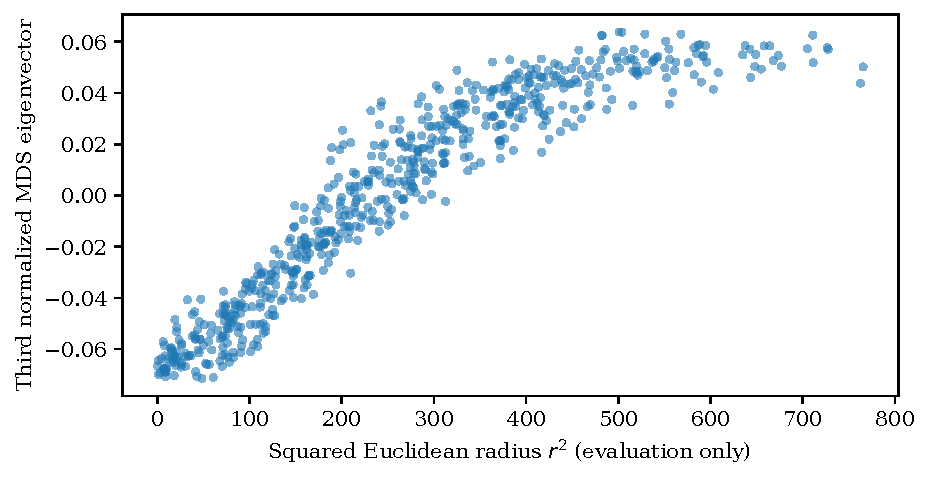
\includegraphics[width=.87\linewidth]{figures/delaunay_bowl.pdf}
\caption{The third hop-MDS eigenvector versus squared radius for the seed-zero Delaunay fixture. Its absolute correlation is $0.930$. Coordinates appear only in this diagnostic; they are not inputs to the hop or SI metric.}
\label{fig:bowl}
\end{figure}

\begin{table}[htbp]
\centering\small
\begin{tabular}{lrrrrr}
\toprule
Metric & $G_2$ & $g_{34}$ & $|\rho(v_3,r^2)|$ & $E_{\rm pair}$ & $E_X$ \\
\midrule
Hop & 0.466 & 5.425 & 0.920 & 0.295 & 0.414 \\
SI & 0.635 & 6.723 & 0.950 & 0.248 & 0.335 \\
Length oracle & 0.895 & 1.182 & 0.267 & 0.016 & 0.018 \\
\bottomrule
\end{tabular}

\caption{New Delaunay comparison, means over all five point-set seeds. $E_{\rm pair}$ is the globally scale-aligned pair-distance error against known Euclidean distances. The oracle is not a graph-intrinsic correction. SI improves several errors but retains a strongly radial, spectrally separated third mode.}
\label{tab:delaunay}
\end{table}

The five-seed mean radial correlation rises from $0.920$ under hop distance to $0.950$ under SI, while the mean $g_{34}$ rises from $5.43$ to $6.72$. The two-mode score improves from $0.466$ to $0.635$, but this is not removal of the bowl. The corresponding mean coordinate error remains $0.335$. A single global scale cannot correct the radial structure.

\subsection{An oracle control and an honest correction target}
For pair-distance evaluation, define $a_*=\langle D,E\rangle_F/\norm{D}_F^2$ and
\begin{equation}
 E_{\rm pair}=\frac{\norm{a_*D-E}_F}{\norm{E}_F}.
\end{equation}
For vertex $i$, average the residual $(a_*D_{ij}-E_{ij})$ over $j$, normalize by the mean of $E$, and aggregate vertices by quartiles of $r_i^2$. Figure~\ref{fig:radial} reports those summaries with sample-standard-deviation bars across the five graphs. The scale fit is an evaluation step, not a change to any edge rule.

\begin{figure}[htbp]
\centering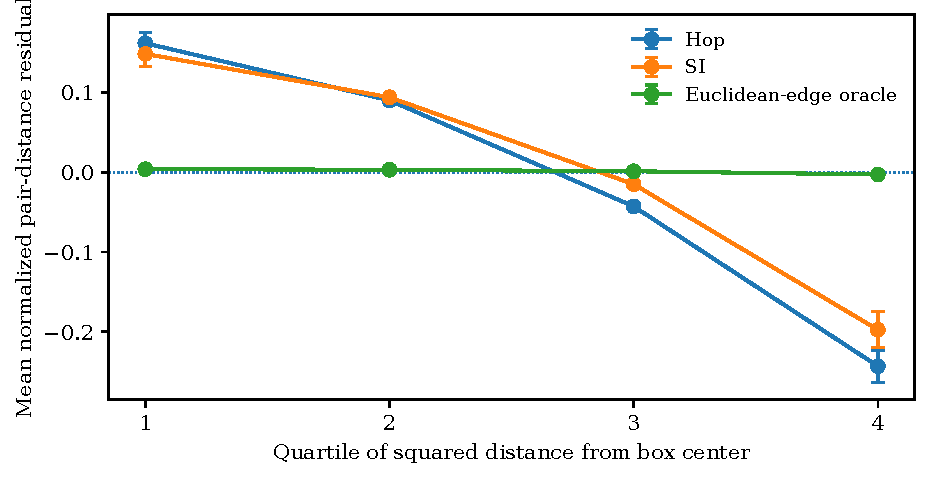
\includegraphics[width=.91\linewidth]{figures/delaunay_radial_residual.pdf}
\caption{Radial structure in pair-distance residuals. SI reduces, but does not eliminate, the systematic center-to-outer-region pattern. Euclidean edge lengths reduce it substantially, while supplying geometric information unavailable to a purely adjacency-based estimator. Error bars describe five-graph sample standard deviations, not independent errors for individual vertex pairs.}
\label{fig:radial}
\end{figure}

The Euclidean-length oracle yields mean pair-distance error $0.0165$ and coordinate error $0.0177$. This is a useful positive control: the triangulation can support a substantially better metric when edge lengths are supplied. Every oracle path has length at least its Euclidean endpoint separation by the Euclidean triangle inequality, so it also admits an exact no-contraction certificate against $E$. Nevertheless, graph detours leave a small residual error. The oracle does not prove that those lengths can be inferred from the unweighted graph or generated by the chosen SI law.

A proposed graph-internal correction should modify edge variables before propagation, or otherwise preserve metric axioms by construction, and then be tested on held-out seeds, sizes, and domain shapes. Removing the third MDS component after inspection is not such a correction. Nor is arbitrary pairwise radial normalization: on a three-point path with distances $(d_{12},d_{23},d_{13})=(1,1,2)$, the transformation $d'_{ij}=d_{ij}/\sqrt{s_i s_j}$ with $(s_1,s_2,s_3)=(1,100,1)$ gives $(0.1,0.1,2)$, violating the triangle inequality.

The coordinate-free elimination of the Delaunay bowl is therefore an explicit unsatisfied validation target in this study. Retaining that result prevents the successful square-grid SI calibration from being mistaken for substrate-independent reconstruction.

\section{Discussion and conclusion}\label{sec:conclusion}
The binary/weighted distinction is not a dichotomy between impossible and inevitable geometry. Binary adjacency can approximate a continuum under a specified scaling, but it cannot by itself express continuously changing interactions on an unchanged finite graph. Dense unit-cost shortcuts can erase reference spatial contrast, yet the resulting MDS failure need not be rank two and need not occur after every added shortcut. Complete-graph equidistance and the new one-swap control make those limitations exact and concrete.

The constructive result is a conditional recovery framework. Shared random edge fields yield finite-sample SI metrics without symmetrization repairs. On an intact finite backbone, weakening finitely many added interactions recovers the backbone's mean metric, and controlled metric errors imply controlled centered Gram matrices. The numerical weak-shortcut experiment illustrates that mechanism. Independent one-, two-, and three-dimensional fixtures test reconstruction against known geometry rather than claiming to derive dimension from the desired output.

Three boundaries remain decisive. Deterministic mean edge costs do not certify mean first-passage distances. A static minimum-cost coarsening rule is not a closed SI renormalization transformation. A finite spectral improvement is not a proof of global Euclidean geometry, boundary uniformity, or manifold convergence. Even a correct intrinsic metric on a curved manifold need not have a globally rank-$d$ Euclidean MDS realization; intrinsic dimension and global embedding dimension are different quantities.

D11 and D10b fit within this framework without being conflated. D11 records weighted finite-window tail behavior whose interpretation depends on volume-ratio recovery and a separately specified propagation law. D10b identifies an inclusion-interface curvature signature, not the absence of boundaries. The Delaunay transfer test then supplies a direct falsifier of the strongest universal reconstruction claim: uniform SI improves several measures but leaves a radial artifact, while a coordinate oracle demonstrates a substantially better attainable control.

The resulting research program has a precise next acceptance condition: derive or independently select an intrinsic local interaction rule, keep it fixed across substrate families and domain shapes, and show that its metric, spectral, coordinate, and boundary diagnostics all meet declared tolerances. The theorems proved here identify what follows once the relevant metric control is obtained. They do not replace that empirical and analytical task with an assumed ontology or a tuned embedding.

\appendix
\section{Reproducibility and source provenance}\label{app:repro}
The accompanying project contains native \LaTeX{} source, figures, tables, JSON result files, compressed distance matrices, realized edge lists, numerical scripts, and an editorial claim audit. It follows the first paper's article-scale typography, numeric citations, and two-pass \texttt{pdflatex} build, while using editable native \TeX{} as the canonical manuscript rather than requiring a Markdown-to-\TeX{} conversion.

The first paper's manuscript and build materials were reviewed, along with selected model notes, the deferred-work ledger, and the graph, weighting, SI, MDS, and dimension-test implementations on the specifically requested branch. This was a targeted source review, not a clone-and-run verification of the entire repository. No upstream commit hash was independently resolved. The branch reference and access date are recorded instead; the exact new code, configurations, and outputs in this package have their own content-hash manifest. An upstream branch may subsequently change.

The new experiments are independent implementations, not copied historical result files. In particular, the static damage graph has 27 detour-classified longs rather than the branch fixture's documented 30; the connected-swap coarsening graph is version-sensitive; the disk samples use a different random-generator family; and SI uses common edge fields rather than independently sampled source rows. These differences are explicit and are not hidden behind a claim of historical numerical reproduction.

The execution environment was Python 3.13.5, NumPy 2.3.5, SciPy 1.17.0, NetworkX 3.6.1, and the Matplotlib version recorded in the requirements file. All graph distances are computed with nonnegative-cost sparse shortest-path routines. MDS uses direct double-centering and symmetric eigendecomposition. A relative numerical eigenvalue tolerance of $10^{-10}$ times $\max(1,\max_i|\lambda_i|)$ is used for sign/rank classification; the unit floor affects only very small overall scales and is not active for the reported principal benchmarks. Edge-census comparisons use $10^{-10}$ tolerance, whereas the integer and dyadic arrival-event values in the certified static tests are compared without radius merging.

The configuration files record graph sizes, seeds, rates, trial counts, and evaluation choices. The SI grid replication uncertainty reflects Monte Carlo variation on one fixed graph. The Delaunay averages and error bars reflect variation over five graph seeds, with one SI Monte Carlo estimator per graph. Pairwise entries from a common graph or field are dependent and are not treated as independent observations.

The deterministic verification script checks complete-graph spectra, the rescaled path, shell formulas, exact intact-backbone recovery under admissible deterministic prices, a tree SI control, and the geometric triangle example. The latter also has a 200,000-trial Monte Carlo cross-check with its standard error saved. These checks are guards for the implementation, not substitutes for the mathematical proofs.

A complete regeneration uses:
\begin{verbatim}
python -m pip install -r requirements.txt
bash build.sh --recompute
\end{verbatim}
A document-only rebuild, using the included verified results and figures, uses \texttt{bash build.sh}. No external research repository is needed to execute the supplied calculations. The README gives separate commands for the primary and secondary numerical batches and specifies which statements are source-reported only.

\clearpage
\section{Prospective acceptance ledger}\label{app:ledger}
\begin{longtable}{>{\raggedright\arraybackslash}p{.23\linewidth}>{\raggedright\arraybackslash}p{.32\linewidth}>{\raggedright\arraybackslash}p{.37\linewidth}}
\toprule
Claim & Evidence in this paper & Remaining condition for a stronger claim \\
\midrule
\endfirsthead
\toprule Claim & Evidence in this paper & Remaining condition for a stronger claim \\\midrule
\endhead
Binary shortcut failure & Exact equidistance result and finite damage examples & A specified ensemble and limit for any universal shortcut threshold. \\
Continuous weighted $L_0$ necessity & Fixed-topology parameterization argument; binary continuum counterexample & Derivation of physical microscopic state and its update law. \\
SI distance validity & Pathwise, expectation, and finite-sample metric proofs & Other directed or history-dependent dynamics require separate analysis. \\
Weak-shortcut restoration & Finite intact-backbone theorem and coupled experiment & Uniform control for growing graphs and a justified geometric baseline. \\
Weighted RG & Static coordinate-block pricing pilot & Dynamical closure, scale conventions, and a fixed-point or convergence analysis. \\
D11 tail closure & Source-reported finite-window diagnostics and exact ratio identities & Independently fixed SI law, event-radius reanalysis, and controlled large-domain tests. \\
D10b disk confirmation & New inclusion-interface curvature measurements & A separate flat-domain reconstruction and boundary-uniformity test. \\
Delaunay correction & Radial diagnostic, failed uniform-SI transfer, and length oracle & A coordinate-free rule that passes held-out metric and boundary tests. \\
General $d$-manifold recovery & Conditional MDS theorem and $d=1,2,3$ controls & Sampling/metric consistency and appropriate local or global embedding assumptions. \\
\bottomrule
\end{longtable}

\clearpage
\begin{thebibliography}{99}
\bibitem{leblond2026a}
P. Leblond, \emph{Distance, Volume, and Apparent Dimension in Weighted Graphs: Exact diagnostics and counterexamples}, September 29, 2026. Manuscript and reproducibility materials. \url{https://github.com/pleblond/weighted-graph-paper}. Accessed September 30, 2026.

\bibitem{leblondBranch}
P. Leblond, \emph{alltoall-black-holes}, research software and model notes, branch \texttt{cursor/d1-dynamics-u-2031}. \url{https://github.com/pleblond/alltoall-black-holes/tree/cursor/d1-dynamics-u-2031}. Accessed September 30, 2026.

\bibitem{richardson1973}
D. Richardson, Random growth in a tessellation, \emph{Mathematical Proceedings of the Cambridge Philosophical Society} \textbf{74}(3) (1973), 515--528. \href{https://doi.org/10.1017/S0305004100077288}{doi:10.1017/S0305004100077288}.

\bibitem{vandenberg1993}
J. van den Berg and H. Kesten, Inequalities for the time constant in first-passage percolation, \emph{Annals of Applied Probability} \textbf{3}(1) (1993), 56--80. \href{https://doi.org/10.1214/aoap/1177005507}{doi:10.1214/aoap/1177005507}.

\bibitem{schoenberg1935}
I. J. Schoenberg, Remarks to Maurice Fr\'echet's article ``Sur la d\'efinition axiomatique d'une classe d'espace distanc\'es vectoriellement applicable sur l'espace de Hilbert,'' \emph{Annals of Mathematics} \textbf{36}(3) (1935), 724--732. \href{https://doi.org/10.2307/1968654}{doi:10.2307/1968654}.

\bibitem{tenenbaum2000}
J. B. Tenenbaum, V. de Silva, and J. C. Langford, A global geometric framework for nonlinear dimensionality reduction, \emph{Science} \textbf{290}(5500) (2000), 2319--2323. \href{https://doi.org/10.1126/science.290.5500.2319}{doi:10.1126/science.290.5500.2319}.

\bibitem{arias2020}
E. Arias-Castro, A. Javanmard, and B. Pelletier, Perturbation bounds for Procrustes, classical scaling, and trilateration, with applications to manifold learning, \emph{Journal of Machine Learning Research} \textbf{21}(15) (2020), 1--37. \url{https://jmlr.org/papers/v21/18-720.html}.

\bibitem{leblondWeighted}
P. Leblond, Weighted audit and static coarsening implementation, \texttt{src/bh\_graph/weighted.py} and \texttt{tests/test\_weighted.py}, in \cite{leblondBranch}, specified branch, accessed September 30, 2026.

\bibitem{leblondSI}
P. Leblond, Persistent SI and source-row first-passage estimator, \texttt{src/bh\_graph/scrambling.py}, in \cite{leblondBranch}, specified branch, accessed September 30, 2026.

\bibitem{leblondMDS}
P. Leblond, MDS calibration tests, \texttt{tests/test\_mds.py}, in \cite{leblondBranch}, specified branch, accessed September 30, 2026.

\bibitem{leblondDimTests}
P. Leblond, D11 tail and D10b disk-interface tests, \texttt{tests/test\_emergent\_dim.py}, in \cite{leblondBranch}, specified branch, accessed September 30, 2026.

\bibitem{leblondLedger}
P. Leblond, Deferred-work and evidence ledger, \texttt{docs/DEFERRED.md}, in \cite{leblondBranch}, specified branch, accessed September 30, 2026.

\bibitem{ollivier2009}
Y. Ollivier, Ricci curvature of Markov chains on metric spaces, \emph{Journal of Functional Analysis} \textbf{256}(3) (2009), 810--864. \href{https://doi.org/10.1016/j.jfa.2008.11.001}{doi:10.1016/j.jfa.2008.11.001}. Author manuscript: \url{https://arxiv.org/abs/math/0701886}.

\bibitem{leblondGraphs}
P. Leblond, Substrate graph generators and swap rule, \texttt{src/bh\_graph/graphs.py} and \texttt{src/bh\_graph/update\_rule.py}, in \cite{leblondBranch}, specified branch, accessed September 30, 2026.
\end{thebibliography}
\end{document}
